\section{Tipos de TableSpace que existen en Oracle.} 
\vspace{\baselineskip}
Un tablespace es una unidad lógica de almacenamiento dentro de una base de datos oracle.\\
Es un puente entre el sistema de ficheros del sistema operativo y la base de datos.\\ \\
Cada tablespace se compone de, al menos, un datafile y un datafile solo puede pertenecer a un tablespace.\\
Cada tabla o indice de oracle pertenece a un tablespace, es decir cuando se crea una tabla o indice se crea en un tablespace determinado.\\ \\
Los tablespace son estructuras donde se almacenan los objetos del esquema de la base de datos, tales como tablas, índices, etc. con la particularidad de poderse repartir en varios ficheros. Por tanto, las bases de datos tienes varios tablespaces y estos a su vez varios datafiles. Un datafile sólo pertenece a un tablespace y un tablespace sólo pertenece a una Base de Datos.
\\
\\
\\
\begin{center}
	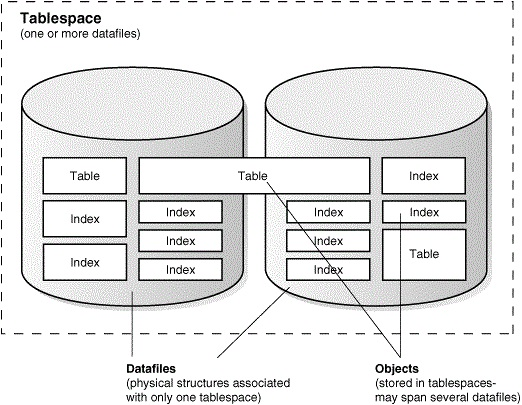
\includegraphics[width=12.5cm]{./Imagenes/4} 
\end{center}

\vspace{\baselineskip}

TIPOS DE TABLESPACE
\\
\\
\begin{itemize}
	\item TABLESPACE SYSTEM:
\end{itemize}
\begin{adjustwidth}{0.40in}{0.0in}
	El espacio de tabla principal en cualquier base de datos es el tablespace SYSTEM, que contiene información básica sobre el funcionamiento del servidor de la base de datos, como el diccionario de datos y el segmento de reversión del sistema. El tablespace SYSTEM es el primer espacio de tabla creado en la creación de la base de datos. Se gestiona como cualquier otro espacio de tabla, pero requiere un mayor nivel de privilegios y está restringido de alguna manera. Por ejemplo, no puede cambiar el nombre o eliminar el tablespace SYSTEM o desconectarlo.	\\ \\
	Características:
	\begin{itemize}
		\item[$*$] Se crea automáticamente al hacer la instalación de Oracle o al crear una Base de Datos.
		\item[$*$] Contiene el diccionario de datos.\\
\\
	\end{itemize}		
\end{adjustwidth}

\begin{itemize}
	\item TABLESPACE TEMPORALES:
\end{itemize}
\begin{adjustwidth}{0.40in}{0.0in}
	Un tablespaces temporal contiene datos transitorios que persisten solo durante la sesión. Los tablespace temporales pueden mejorar la concurrencia de múltiples operaciones de clasificación que no caben en la memoria y pueden mejorar la eficiencia de las operaciones de gestión de espacio durante las clasificaciones.\\ \\
	Los tablespace temporales se utilizan para almacenar lo siguiente:
	\begin{itemize}
		\item[$*$] Resultados de clasificación intermedios.
		\item[$*$] Tablas temporales e índices temporales.
		\item[$*$] LOB's temporales.
		\item[$*$] Árboles B temporales.\\
\\
	\end{itemize}
	Dentro de un espacio de tabla temporal, todas las operaciones de clasificación para una instancia particular comparten un único segmento de clasificación, y existen segmentos de clasificación para cada instancia que realiza operaciones de clasificación que requieren espacio temporal. La primera instrucción después de la puesta en marcha crea un segmento de clasificación que utiliza el espacio de tabla temporal para la clasificación, y se libera solo en el cierre.\\ \\
	Características:
	\begin{itemize}
		\item[$*$] Es aquél en el que solamente puede haber objetos temporales. No se pueden crear objetos permanentes como pueden ser los índices, las tablas o los segmentos de rollback.
		\item[$*$] Optimización operaciones de ordenación.\\
\\
	\end{itemize}		
\end{adjustwidth}

\begin{itemize}
	\item TIPO BIGFILE (10g):
\end{itemize}
\begin{adjustwidth}{0.40in}{0.0in}
	Un tablespace bigfile es un tablespace con un archivo de datos único, pero muy grande (hasta bloques 4G). Los tablespace tradicionales de archivos pequeños, por el contrario, pueden contener varios archivos de datos, pero los archivos no pueden ser tan grandes. Los beneficios de los tablespace de bigfile son los siguientes:
	\begin{itemize}
		\item[$*$] Un espacio de tabla de bigfile con bloques de 8K puede contener un archivo de datos de 32 terabytes. 
		\item[$*$] Los tablespace de bigfile pueden reducir la cantidad de archivos de datos necesarios para una base de datos. 
		\item[$*$] Los tablespace de bigfile simplifican la administración de la base de datos al proporcionar transparencia de archivos de datos. \\
\\
	\end{itemize}
	Los tablespace de Bigfile solo se admiten para tablespace administrados localmente con administración de espacio de segmento automática, con tres excepciones: tablespace deshacer gestionados localmente, tablespace temporales y el tablespace SYSTEM.		
\end{adjustwidth}

\begin{itemize}
	\item TIPO SMALL-FILE (10g):
\end{itemize}
\begin{adjustwidth}{0.40in}{0.0in}
	Utilice esta cláusula para determinar si el espacio de tabla es un espacio de tabla de bigfile o smallfile. Esta cláusula anula cualquier configuración de tipo de espacio de tabla predeterminada para la base de datos.\\ \\		
	Un tablespace SmallFile es un espacio de tabla de Oracle tradicional, que puede contener 1022 archivos de datos o archivos temporales, cada uno de los cuales puede contener hasta aproximadamente 4 millones (2~22)de bloques.\\ \\	
	Un tablespace SmallFile muy diferente de un espacio de tabla de archivo grande.El tablespace SmallFile es el espacio de tabla "tradicional" de Oracle, y la distinción solo se hizo en 10 g con la introducción del tablespace de bigfile.\\ \\	
	El valor predeterminado para los tipos de espacios de tablas es un espacio de tablas de pequeño tamaño, pero el valor predeterminado se puede cambiar al crear la base de datos:\\\\
\\
	\begin{center}
		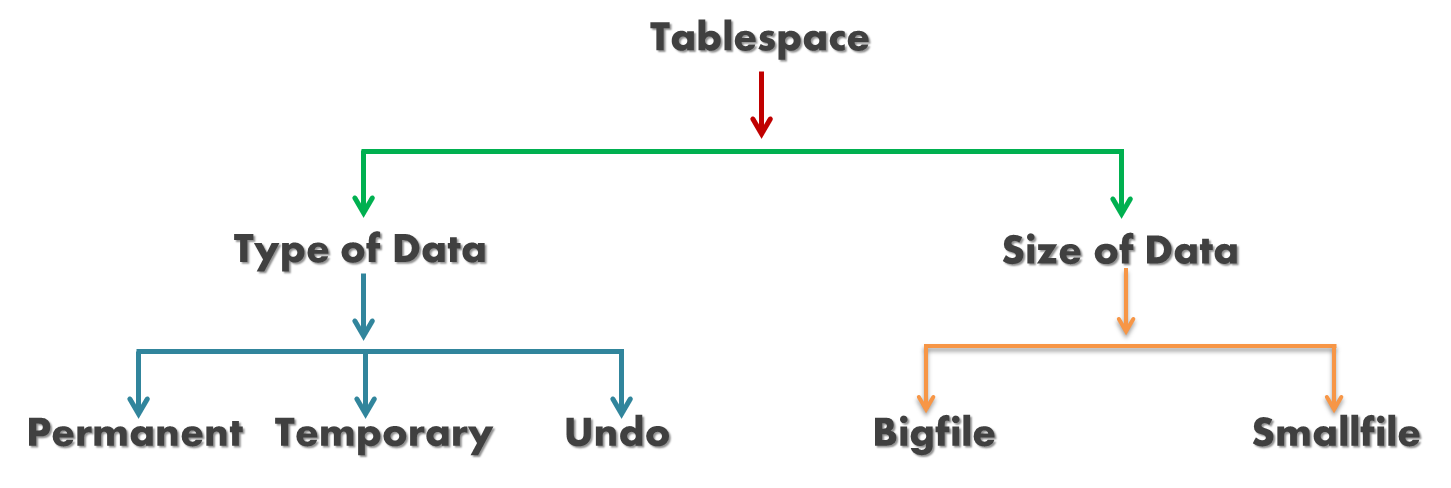
\includegraphics[width=15.3cm]{./Imagenes/5}
	\end{center}
\end{adjustwidth}

\vspace{\baselineskip}

\begin{itemize}
	\item TABLESPACE READ-ONLY:
\end{itemize}
\begin{adjustwidth}{0.40in}{0.0in}
	La creación de un tablespace de solo lectura evita las operaciones de escritura en los archivos de datos en el tablespace. El propósito principal de los espacios de tabla de solo lectura es eliminar la necesidad de realizar copias de seguridad y recuperación de grandes porciones estáticas de una base de datos.\\ \\
	Los espacios de tabla de solo lectura también proporcionan una forma de proteger los datos históricos para que los usuarios no puedan modificarlos. La creación de un tablespace de solo lectura evita actualizaciones en todas las tablas del tablespace, independientemente del nivel de privilegio de actualización del usuario.\\ \\	
	Se pueden consultar los datos de los objetos, no se puede ni borrar ni insertar nada en ellos. La principal ventaja de un tablespace read-only es que no hace falta hacer backup del mismo.\\
\\
\end{adjustwidth}

\vspace{\baselineskip}